\documentclass[conference]{IEEEtran}
%DIF LATEXDIFF DIFFERENCE FILE
%DIF DEL main_v1.tex   Sun Oct 11 18:35:09 2026
%DIF ADD main.tex      Sun Oct 11 18:40:07 2026
\IEEEoverridecommandlockouts
\usepackage[T1]{fontenc}
\usepackage{mathptmx}
\usepackage{cite}
\usepackage{amsmath}
\usepackage{graphicx}
\usepackage{booktabs}
\usepackage[hidelinks]{hyperref}
\newcommand{\usd}{\$}
\makeatletter\newcommand{\tabinput}[1]{\@@input #1 }\makeatother
\newcommand{\maxcovstd}{0.004}
\newcommand{\kappafit}{4.0}

\DeclareMathOperator*{\median}{median}
%DIF PREAMBLE EXTENSION ADDED BY LATEXDIFF
%DIF UNDERLINE PREAMBLE %DIF PREAMBLE
\RequirePackage[normalem]{ulem} %DIF PREAMBLE
\RequirePackage{color}\definecolor{RED}{rgb}{1,0,0}\definecolor{BLUE}{rgb}{0,0,1} %DIF PREAMBLE
\providecommand{\DIFaddtex}[1]{{\protect\color{blue}\uwave{#1}}} %DIF PREAMBLE
\providecommand{\DIFdeltex}[1]{{\protect\color{red}\sout{#1}}}                      %DIF PREAMBLE
%DIF SAFE PREAMBLE %DIF PREAMBLE
\providecommand{\DIFaddbegin}{} %DIF PREAMBLE
\providecommand{\DIFaddend}{} %DIF PREAMBLE
\providecommand{\DIFdelbegin}{} %DIF PREAMBLE
\providecommand{\DIFdelend}{} %DIF PREAMBLE
\providecommand{\DIFmodbegin}{} %DIF PREAMBLE
\providecommand{\DIFmodend}{} %DIF PREAMBLE
%DIF FLOATSAFE PREAMBLE %DIF PREAMBLE
\providecommand{\DIFaddFL}[1]{\DIFadd{#1}} %DIF PREAMBLE
\providecommand{\DIFdelFL}[1]{\DIFdel{#1}} %DIF PREAMBLE
\providecommand{\DIFaddbeginFL}{} %DIF PREAMBLE
\providecommand{\DIFaddendFL}{} %DIF PREAMBLE
\providecommand{\DIFdelbeginFL}{} %DIF PREAMBLE
\providecommand{\DIFdelendFL}{} %DIF PREAMBLE
%DIF HYPERREF PREAMBLE %DIF PREAMBLE
\providecommand{\DIFadd}[1]{\texorpdfstring{\DIFaddtex{#1}}{#1}} %DIF PREAMBLE
\providecommand{\DIFdel}[1]{\texorpdfstring{\DIFdeltex{#1}}{}} %DIF PREAMBLE
\newcommand{\DIFscaledelfig}{0.5}
%DIF HIGHLIGHTGRAPHICS PREAMBLE %DIF PREAMBLE
\RequirePackage{settobox} %DIF PREAMBLE
\RequirePackage{letltxmacro} %DIF PREAMBLE
\newsavebox{\DIFdelgraphicsbox} %DIF PREAMBLE
\newlength{\DIFdelgraphicswidth} %DIF PREAMBLE
\newlength{\DIFdelgraphicsheight} %DIF PREAMBLE
% store original definition of \includegraphics %DIF PREAMBLE
\LetLtxMacro{\DIFOincludegraphics}{\includegraphics} %DIF PREAMBLE
\newcommand{\DIFaddincludegraphics}[2][]{{\color{blue}\fbox{\DIFOincludegraphics[#1]{#2}}}} %DIF PREAMBLE
\newcommand{\DIFdelincludegraphics}[2][]{% %DIF PREAMBLE
\sbox{\DIFdelgraphicsbox}{\DIFOincludegraphics[#1]{#2}}% %DIF PREAMBLE
\settoboxwidth{\DIFdelgraphicswidth}{\DIFdelgraphicsbox} %DIF PREAMBLE
\settoboxtotalheight{\DIFdelgraphicsheight}{\DIFdelgraphicsbox} %DIF PREAMBLE
\scalebox{\DIFscaledelfig}{% %DIF PREAMBLE
\parbox[b]{\DIFdelgraphicswidth}{\usebox{\DIFdelgraphicsbox}\\[-\baselineskip] \rule{\DIFdelgraphicswidth}{0em}}\llap{\resizebox{\DIFdelgraphicswidth}{\DIFdelgraphicsheight}{% %DIF PREAMBLE
\setlength{\unitlength}{\DIFdelgraphicswidth}% %DIF PREAMBLE
\begin{picture}(1,1)% %DIF PREAMBLE
\thicklines\linethickness{2pt} %DIF PREAMBLE
{\color[rgb]{1,0,0}\put(0,0){\framebox(1,1){}}}% %DIF PREAMBLE
{\color[rgb]{1,0,0}\put(0,0){\line( 1,1){1}}}% %DIF PREAMBLE
{\color[rgb]{1,0,0}\put(0,1){\line(1,-1){1}}}% %DIF PREAMBLE
\end{picture}% %DIF PREAMBLE
}\hspace*{3pt}}} %DIF PREAMBLE
} %DIF PREAMBLE
\LetLtxMacro{\DIFOaddbegin}{\DIFaddbegin} %DIF PREAMBLE
\LetLtxMacro{\DIFOaddend}{\DIFaddend} %DIF PREAMBLE
\LetLtxMacro{\DIFOdelbegin}{\DIFdelbegin} %DIF PREAMBLE
\LetLtxMacro{\DIFOdelend}{\DIFdelend} %DIF PREAMBLE
\DeclareRobustCommand{\DIFaddbegin}{\DIFOaddbegin \let\includegraphics\DIFaddincludegraphics} %DIF PREAMBLE
\DeclareRobustCommand{\DIFaddend}{\DIFOaddend \let\includegraphics\DIFOincludegraphics} %DIF PREAMBLE
\DeclareRobustCommand{\DIFdelbegin}{\DIFOdelbegin \let\includegraphics\DIFdelincludegraphics} %DIF PREAMBLE
\DeclareRobustCommand{\DIFdelend}{\DIFOaddend \let\includegraphics\DIFOincludegraphics} %DIF PREAMBLE
\LetLtxMacro{\DIFOaddbeginFL}{\DIFaddbeginFL} %DIF PREAMBLE
\LetLtxMacro{\DIFOaddendFL}{\DIFaddendFL} %DIF PREAMBLE
\LetLtxMacro{\DIFOdelbeginFL}{\DIFdelbeginFL} %DIF PREAMBLE
\LetLtxMacro{\DIFOdelendFL}{\DIFdelendFL} %DIF PREAMBLE
\DeclareRobustCommand{\DIFaddbeginFL}{\DIFOaddbeginFL \let\includegraphics\DIFaddincludegraphics} %DIF PREAMBLE
\DeclareRobustCommand{\DIFaddendFL}{\DIFOaddendFL \let\includegraphics\DIFOincludegraphics} %DIF PREAMBLE
\DeclareRobustCommand{\DIFdelbeginFL}{\DIFOdelbeginFL \let\includegraphics\DIFdelincludegraphics} %DIF PREAMBLE
\DeclareRobustCommand{\DIFdelendFL}{\DIFOaddendFL \let\includegraphics\DIFOincludegraphics} %DIF PREAMBLE
%DIF COLORLISTINGS PREAMBLE %DIF PREAMBLE
\RequirePackage{listings} %DIF PREAMBLE
\RequirePackage{color} %DIF PREAMBLE
\lstdefinelanguage{DIFcode}{ %DIF PREAMBLE
%DIF DIFCODE_UNDERLINE %DIF PREAMBLE
  moredelim=[il][\color{red}\sout]{\%DIF\ <\ }, %DIF PREAMBLE
  moredelim=[il][\color{blue}\uwave]{\%DIF\ >\ } %DIF PREAMBLE
} %DIF PREAMBLE
\lstdefinestyle{DIFverbatimstyle}{ %DIF PREAMBLE
	language=DIFcode, %DIF PREAMBLE
	basicstyle=\ttfamily, %DIF PREAMBLE
	columns=fullflexible, %DIF PREAMBLE
	keepspaces=true %DIF PREAMBLE
} %DIF PREAMBLE
\lstnewenvironment{DIFverbatim}{\lstset{style=DIFverbatimstyle}}{} %DIF PREAMBLE
\lstnewenvironment{DIFverbatim*}{\lstset{style=DIFverbatimstyle,showspaces=true}}{} %DIF PREAMBLE
%DIF END PREAMBLE EXTENSION ADDED BY LATEXDIFF

\begin{document}

\title{Conformal Uncertainty Quantification for Physics-Informed American Option Pricing: The Difficulty Score Must Respect Complementarity}

\author{\IEEEauthorblockN{Gaurang Gupta, Arush Gupta, Utkarsh Nigam}
\IEEEauthorblockA{Mukesh Patel School of Technology Management and Engineering (MPSTME)\\
SVKM's NMIMS (Deemed-to-be University), Vile Parle (W), Mumbai 400056, India\\
Email: [GAURANG\_EMAIL] (corresponding author), [ARUSH\_EMAIL], [UTKARSH\_EMAIL]}}

\maketitle

\begin{abstract}
Physics-informed neural networks (PINNs) can price options without labelled prices, but a point price is not a risk number. We study split conformal prediction on top of PINN pricers for European and American puts under geometric Brownian motion, with exact Black-Scholes and 500-step binomial prices as calibration and test labels. Over ten training seeds, the PDE loss cuts the European mean absolute error from \usd 4.42 (a control without the PDE term) to \usd 0.25 and shrinks the 90\% split-conformal band from \usd 19.43 to \usd 0.94. Labelled regressors are more accurate inside their training region, but kernel and polynomial ridge fail outside it. Split conformal reaches nominal marginal coverage for every model, including an American PINN that overprices by \usd 3.13 on average: the bias costs width, not coverage. The raw PDE residual is uninformative for the American put (rank correlation $-0.01$) and widens the band, in part because a positive residual is correct in the exercise region. The complementarity residual $\min(L[u],u-h)$ tracks the error (rank correlation 0.77) and narrows the band from \usd 10.05 to \usd 9.01 at equal coverage. Mondrian buckets give the best worst-bucket coverage (0.86 against 0.71). All labels are synthetic; we claim no market coverage.
\end{abstract}

\begin{IEEEkeywords}
physics-informed neural networks, American options, conformal prediction, uncertainty quantification, no-arbitrage
\end{IEEEkeywords}

\section{Introduction}
A trader who receives a model price also needs to know how far that price may be from the truth. A price without a band is not a risk number. \DIFdelbegin \DIFdel{For American options the problem is harder than for European ones, since the early-exercise boundary is unknown and no closed form }\DIFdelend \DIFaddbegin \DIFadd{An American contract adds a second difficulty. Its holder can exercise early, the exercise boundary has to be found as part of the solution, and no closed-form price }\DIFaddend exists \cite{merton1973theory,hull2022options}. \DIFdelbegin \DIFdel{Lattice and simulation methods give accurate references \mbox{%DIFAUXCMD
\cite{cox1979option,longstaff2001valuing}}\hskip0pt%DIFAUXCMD
, but they do not say how wrong }\DIFdelend \DIFaddbegin \DIFadd{Trees and Monte Carlo produce accurate reference values \mbox{%DIFAUXCMD
\cite{cox1979option,longstaff2001valuing}}\hskip0pt%DIFAUXCMD
. They cannot tell us, however, the error of }\DIFaddend a fast surrogate \DIFdelbegin \DIFdel{is at a new }\DIFdelend \DIFaddbegin \DIFadd{at an unseen }\DIFaddend point. Learned pricers bring two further issues. Regressors trained on labelled prices need many labels and can break calendar or convexity conditions. PINNs need no labels \cite{raissi2019physics}, but their error is not known in advance.

This paper puts distribution-free conformal bands \cite{vovk2005algorithmic,lei2018distribution} around PINN pricers and asks which difficulty score should scale the band. Our contributions are as follows.
\begin{enumerate}
\item A controlled study of split, residual-normalised and Mondrian conformal prediction on a European PINN (N1), its no-physics control (N0), and an American PINN (N2), over 10 training seeds and 20 calibration splits each.
\item Evidence that the raw PDE residual $|L[u]|$ is a poor difficulty score for the American put, and that the complementarity residual $|\min(L[u],u-h)|$ is a good one. The residual has to follow the structure of the problem.
\item A labelled-baseline comparison and a static-arbitrage check of PINN prices and of interval edges, both reported without repair.
\end{enumerate}
We state the limits at the outset. All labels are synthetic and exact. Our American PINN has a systematic upward bias of \usd 3.13 on a \usd 100 strike. We report no coverage on market quotes.

\section{Related Work}
\emph{\DIFdelbegin \DIFdel{Classical pricing}\DIFdelend \DIFaddbegin \DIFadd{Reference pricers}\DIFaddend .} \DIFdelbegin \DIFdel{The Black-Scholes model \mbox{%DIFAUXCMD
\cite{black1973pricing}}\hskip0pt%DIFAUXCMD
and }\DIFdelend \DIFaddbegin \DIFadd{Our European ground truth is the closed-form price of \mbox{%DIFAUXCMD
\cite{black1973pricing}}\hskip0pt%DIFAUXCMD
. The no-arbitrage conditions we test come from }\DIFaddend Merton's \DIFdelbegin \DIFdel{rational bounds \mbox{%DIFAUXCMD
\cite{merton1973theory}}\hskip0pt%DIFAUXCMD
give the European price and the no-arbitrage conditions we test. The binomial lattice of Cox, Ross and Rubinstein \mbox{%DIFAUXCMD
\cite{cox1979option}}\hskip0pt%DIFAUXCMD
handles early exercise and serves here as the American reference. Barone-Adesi and Whaley \mbox{%DIFAUXCMD
\cite{baroneadesi1987efficient} }\hskip0pt%DIFAUXCMD
give a fast analytic approximation , and Longstaff and Schwartz \mbox{%DIFAUXCMD
\cite{longstaff2001valuing}}\hskip0pt%DIFAUXCMD
price American options by least-squares Monte Carlo. Stochastic volatility models \mbox{%DIFAUXCMD
\cite{heston1993closed}}\hskip0pt%DIFAUXCMD
are usually solved with finite differences, for example ADI schemes \mbox{%DIFAUXCMD
\cite{inthout2010adi} }\hskip0pt%DIFAUXCMD
}\DIFdelend \DIFaddbegin \DIFadd{bounds \mbox{%DIFAUXCMD
\cite{merton1973theory}}\hskip0pt%DIFAUXCMD
. For the American put we use the recombining tree of \mbox{%DIFAUXCMD
\cite{cox1979option}}\hskip0pt%DIFAUXCMD
, which compares holding and exercising at every node. Two other routes exist: a quadratic analytic approximation \mbox{%DIFAUXCMD
\cite{baroneadesi1987efficient}}\hskip0pt%DIFAUXCMD
, and simulation in which a regression estimates the value of continuing \mbox{%DIFAUXCMD
\cite{longstaff2001valuing}}\hskip0pt%DIFAUXCMD
}\DIFaddend . \DIFdelbegin \DIFdel{Textbook treatments of }\DIFdelend \DIFaddbegin \DIFadd{Under stochastic volatility \mbox{%DIFAUXCMD
\cite{heston1993closed}}\hskip0pt%DIFAUXCMD
, grid methods such as ADI splitting \mbox{%DIFAUXCMD
\cite{inthout2010adi} }\hskip0pt%DIFAUXCMD
are a common choice. Standard texts such as \mbox{%DIFAUXCMD
\cite{hull2022options} }\hskip0pt%DIFAUXCMD
cover put-call }\DIFaddend parity and early exercise\DIFdelbegin \DIFdel{are in \mbox{%DIFAUXCMD
\cite{hull2022options}}\hskip0pt%DIFAUXCMD
}\DIFdelend .

\emph{\DIFdelbegin \DIFdel{Neural }\DIFdelend \DIFaddbegin \DIFadd{Networks as }\DIFaddend PDE solvers.} \DIFdelbegin \DIFdel{PINNs train a network so that a PDEresidual, boundary terms and an }\DIFdelend \DIFaddbegin \DIFadd{A PINN \mbox{%DIFAUXCMD
\cite{raissi2019physics} }\hskip0pt%DIFAUXCMD
is fitted by penalising, at random points, how far it is from satisfying the PDE, its boundary values and its }\DIFaddend initial or terminal \DIFdelbegin \DIFdel{term are small at sampled points \mbox{%DIFAUXCMD
\cite{raissi2019physics}}\hskip0pt%DIFAUXCMD
. The Deep Galerkin Method \mbox{%DIFAUXCMD
\cite{sirignano2018dgm} }\hskip0pt%DIFAUXCMD
follows a similar }\DIFdelend \DIFaddbegin \DIFadd{value. DGM \mbox{%DIFAUXCMD
\cite{sirignano2018dgm} }\hskip0pt%DIFAUXCMD
is a close }\DIFaddend mesh-free \DIFdelbegin \DIFdel{idea }\DIFdelend \DIFaddbegin \DIFadd{relative }\DIFaddend and includes an American option \DIFdelbegin \DIFdel{example, and the deep BSDE method \mbox{%DIFAUXCMD
\cite{han2018solving} }\hskip0pt%DIFAUXCMD
targets high-dimensional PDEs . Applied work has used PINNs for }\DIFdelend \DIFaddbegin \DIFadd{among its tests. The deep BSDE solver \mbox{%DIFAUXCMD
\cite{han2018solving} }\hskip0pt%DIFAUXCMD
aims at PDEs in many dimensions. In finance, PINN variants have priced contracts under }\DIFaddend Black-Scholes type equations \cite{bai2022application}, \DIFdelbegin \DIFdel{for American options \mbox{%DIFAUXCMD
\cite{gatta2023meshless} }\hskip0pt%DIFAUXCMD
and for the Heston model \mbox{%DIFAUXCMD
\cite{hainaut2024option}}\hskip0pt%DIFAUXCMD
. To our knowledge, these studies focus on point accuracy rather than on }\DIFdelend \DIFaddbegin \DIFadd{with early exercise \mbox{%DIFAUXCMD
\cite{gatta2023meshless} }\hskip0pt%DIFAUXCMD
and under Heston dynamics \mbox{%DIFAUXCMD
\cite{hainaut2024option}}\hskip0pt%DIFAUXCMD
. As far as we can tell, these papers measure price accuracy and do not report }\DIFaddend calibrated error bands.

\emph{\DIFdelbegin \DIFdel{Labelled learners and shape constraints}\DIFdelend \DIFaddbegin \DIFadd{Learners trained on prices}\DIFaddend .} \DIFdelbegin \DIFdel{Tree ensembles \mbox{%DIFAUXCMD
\cite{ho1995random,breiman2001random} }\hskip0pt%DIFAUXCMD
and gradient boosting \mbox{%DIFAUXCMD
\cite{friedman2001greedy} }\hskip0pt%DIFAUXCMD
are strong tabular regressors. Input-convex networks \mbox{%DIFAUXCMD
\cite{amos2017input} }\hskip0pt%DIFAUXCMD
build convexity into the architecture, which matches the convexity of option prices }\DIFdelend \DIFaddbegin \DIFadd{For tabular data, random forests \mbox{%DIFAUXCMD
\cite{ho1995random,breiman2001random} }\hskip0pt%DIFAUXCMD
and boosted trees \mbox{%DIFAUXCMD
\cite{friedman2001greedy} }\hskip0pt%DIFAUXCMD
are standard, well-tested choices. An input-convex network \mbox{%DIFAUXCMD
\cite{amos2017input} }\hskip0pt%DIFAUXCMD
is convex in chosen inputs by design, and option prices are convex }\DIFaddend in the underlying.

\emph{\DIFdelbegin \DIFdel{Conformal prediction}\DIFdelend \DIFaddbegin \DIFadd{Distribution-free bands}\DIFaddend .} \DIFdelbegin \DIFdel{Conformal prediction gives finite-sample coverage under exchangeability \mbox{%DIFAUXCMD
\cite{vovk2005algorithmic}}\hskip0pt%DIFAUXCMD
. The inductive or split version uses a held-out calibration set \mbox{%DIFAUXCMD
\cite{papadopoulos2002inductive}}\hskip0pt%DIFAUXCMD
, and its regression guarantee is analysed in \mbox{%DIFAUXCMD
\cite{lei2018distribution} }\hskip0pt%DIFAUXCMD
. Normalised scores divide the residual by a local difficulty estimate \mbox{%DIFAUXCMD
\cite{papadopoulos2011regression}}\hskip0pt%DIFAUXCMD
. Conformalized quantile regression \mbox{%DIFAUXCMD
\cite{romano2019conformalized} }\hskip0pt%DIFAUXCMD
adapts width through quantile models, and Mondrian conformal regressors \mbox{%DIFAUXCMD
\cite{bostrom2020mondrian} }\hskip0pt%DIFAUXCMD
calibrate inside categories. A tutorial is given in \mbox{%DIFAUXCMD
\cite{angelopoulos2023conformal} }\hskip0pt%DIFAUXCMD
}\DIFdelend \DIFaddbegin \DIFadd{When the data are exchangeable, a conformal set contains the truth with a stated probability for any sample size \mbox{%DIFAUXCMD
\cite{vovk2005algorithmic}}\hskip0pt%DIFAUXCMD
. A cheap variant fits the model once and sets the band width from residuals on points kept aside \mbox{%DIFAUXCMD
\cite{papadopoulos2002inductive}}\hskip0pt%DIFAUXCMD
; Lei et al.~\mbox{%DIFAUXCMD
\cite{lei2018distribution} }\hskip0pt%DIFAUXCMD
study what this variant guarantees for regression. Scaling each residual by an estimate of local difficulty makes the band width vary from point to point \mbox{%DIFAUXCMD
\cite{papadopoulos2011regression}}\hskip0pt%DIFAUXCMD
. CQR \mbox{%DIFAUXCMD
\cite{romano2019conformalized} }\hskip0pt%DIFAUXCMD
gets a similar effect from quantile models. Mondrian regressors \mbox{%DIFAUXCMD
\cite{bostrom2020mondrian} }\hskip0pt%DIFAUXCMD
repeat the calibration within each group of inputs. Angelopoulos and Bates \mbox{%DIFAUXCMD
\cite{angelopoulos2023conformal} }\hskip0pt%DIFAUXCMD
give an accessible overview}\DIFaddend .

\emph{Gap.} We found no study that uses the physics residual of a PINN pricer as the conformal difficulty score, and none that asks whether that residual is valid for a free-boundary problem.

\section{Method}
\subsection{Pricing problem}
\DIFdelbegin \DIFdel{Let }\DIFdelend \DIFaddbegin \DIFadd{We write }\DIFaddend $S$ \DIFdelbegin \DIFdel{be the spot , }\DIFdelend \DIFaddbegin \DIFadd{for the spot price and }\DIFaddend $K$ \DIFdelbegin \DIFdel{the strike, }\DIFdelend \DIFaddbegin \DIFadd{for the strike. Time to expiry is }\DIFaddend $\tau=T-t$\DIFdelbegin \DIFdel{the time to expiry , $r$ the rate, $q$ the }\DIFdelend \DIFaddbegin \DIFadd{. The interest rate, }\DIFaddend dividend yield and \DIFdelbegin \DIFdel{$\sigma$ the volatility . We use }\DIFdelend \DIFaddbegin \DIFadd{volatility are $r$, $q$ and $\sigma$. With }\DIFaddend moneyness $m=S/K$ and \DIFdelbegin \DIFdel{the price in strike units }\DIFdelend \DIFaddbegin \DIFadd{price per unit strike }\DIFaddend $u(m,\tau)=V/K$\DIFdelbegin \DIFdel{. The Black-Scholes operator \mbox{%DIFAUXCMD
\cite{black1973pricing,merton1973theory} }\hskip0pt%DIFAUXCMD
in these coordinates is
}\DIFdelend \DIFaddbegin \DIFadd{, the pricing operator of \mbox{%DIFAUXCMD
\cite{black1973pricing,merton1973theory} }\hskip0pt%DIFAUXCMD
reads
}\DIFaddend \begin{equation}
L[u]=u_\tau-(r-q)\,m\,u_m-\tfrac12\sigma^2m^2u_{mm}+r\,u. \label{eq:op}
\end{equation}
A European put solves $L[u]=0$ with $u(m,0)=h(m)=\max(1-m,0)$, $u(0,\tau)=e^{-r\tau}$ and $u(m_{\max},\tau)=0$. The American put solves the linear complementarity problem (LCP)
\begin{equation}
L[u]\ge0,\qquad u\ge h,\qquad L[u]\,(u-h)=0. \label{eq:lcp}
\end{equation}
In the exercise region $u=h=1-m$, and (\ref{eq:op}) gives $L[h]=r-q\,m$, which equals $r>0$ when $q=0$. So a positive $L[u]$ there is correct, not an error.

\subsection{Networks and losses}
Each PINN is a tanh multilayer perceptron with 4 hidden layers of 64 units on input $(m,\tau)$. \DIFdelbegin \DIFdel{We use tanh because the residual needs }\DIFdelend \DIFaddbegin \DIFadd{The residual contains }\DIFaddend $u_{mm}$\DIFdelbegin \DIFdel{, and the second derivative of a }\DIFdelend \DIFaddbegin \DIFadd{. A }\DIFaddend ReLU network is \DIFdelbegin \DIFdel{zero almost everywhere. Derivatives come from automatic differentiation in }\DIFdelend \DIFaddbegin \DIFadd{piecewise linear, so this term would vanish except on a set of measure zero; tanh avoids the problem. We obtain $u_m$, $u_{mm}$ and $u_\tau$ with the automatic differentiation of }\DIFaddend PyTorch \cite{paszke2019pytorch}. Let $\overline{(\cdot)}$ denote a mean over points resampled every epoch: 3000 interior points on $[0,3]\times[0,1]$, 400 terminal points (half of them near $m=1$) and 200 boundary points. The European loss is
\begin{equation}
\mathcal L_{\mathrm{E}}=\lambda_{p}\,\overline{L[u]^2}+3\,\overline{(u-h)^2}_{\tau=0}+\overline{(u-g)^2}_{\partial}, \label{eq:le}
\end{equation}
where $g$ is the boundary value. N1 uses $\lambda_p=1$. N0 uses $\lambda_p=0$, so it fits only the payoff and the edges; it is the control. The American loss N2 replaces the PDE term with three LCP penalties, each with weight 1,
\begin{equation}
\overline{\mathrm{relu}(-L[u])^2}+\overline{\mathrm{relu}(h-u)^2}+\overline{(L[u](u-h))^2}, \label{eq:la}
\end{equation}
plus the same terminal and boundary terms. All runs use fixed weights. Training uses Adam with learning rate $2\times10^{-3}$, halved every 2000 of 6000 epochs. The PINNs see no labelled price.

\subsection{Labelled baselines}
Table~\ref{tab:base} lists ten labelled regressors from an earlier project run. They learn $(m,\tau)\mapsto u$ from 500-step binomial labels \cite{cox1979option}. The four classical models use scikit-learn \cite{pedregosa2011scikit} and the six networks use PyTorch.

\subsection{Conformal intervals}
Let $\hat u$ be a PINN prediction and $R(m,\tau)$ a signed residual. On $n$ calibration points with exact labels we compute
\begin{equation}
s_i=\frac{|u_i-\hat u_i|}{1+\kappa|R_i|},\qquad \kappa=\frac{1}{\median_i|R_i|}. \label{eq:score}
\end{equation}
With $\kappa=0$ this is split conformal \cite{papadopoulos2002inductive}; with $\kappa>0$ it is a normalised score \cite{papadopoulos2011regression}. \DIFdelbegin \DIFdel{Let }\DIFdelend \DIFaddbegin \DIFadd{Sort the scores and take }\DIFaddend $q$ \DIFdelbegin \DIFdel{be the $k$-th smallest score with
}\DIFdelend \DIFaddbegin \DIFadd{as the one in position
}\DIFaddend \begin{equation}
k=\lceil (n+1)(1-\alpha)\rceil , \label{eq:k}
\end{equation}
\DIFdelbegin \DIFdel{which }\DIFdelend \DIFaddbegin \DIFadd{counting from the smallest. This rank }\DIFaddend is the finite-sample \DIFdelbegin \DIFdel{quantile }\DIFdelend \DIFaddbegin \DIFadd{correction }\DIFaddend of split conformal \cite{lei2018distribution}. \DIFdelbegin \DIFdel{The band in dollars at }\DIFdelend \DIFaddbegin \DIFadd{At }\DIFaddend a test point\DIFdelbegin \DIFdel{is
}\DIFdelend \DIFaddbegin \DIFadd{, the dollar band is
}\DIFaddend \begin{equation}
\DIFdelbegin %DIFDELCMD < \big[%%%
\DIFdelend K\hat \DIFdelbegin \DIFdel{u-Kq(1+\kappa|R|),}\DIFdelend \DIFaddbegin \DIFadd{u-w\;}\le\DIFadd{\;V\;}\le\DIFaddend \;K\hat u+\DIFaddbegin \DIFadd{w,}\qquad \DIFadd{w=}\DIFaddend Kq\DIFaddbegin \DIFadd{\,}\DIFaddend (1+\kappa|R|)\DIFdelbegin %DIFDELCMD < \big]%%%
\DIFdelend . \label{eq:band}
\end{equation}
\DIFdelbegin \DIFdel{If }\DIFdelend \DIFaddbegin \DIFadd{Under exchangeable }\DIFaddend calibration and test points\DIFdelbegin \DIFdel{are exchangeable, the band covers }\DIFdelend \DIFaddbegin \DIFadd{, the chance that this band misses }\DIFaddend the true price \DIFdelbegin \DIFdel{with probability at least $1-\alpha$ }\DIFdelend \DIFaddbegin \DIFadd{is at most $\alpha$ }\DIFaddend \cite{lei2018distribution}. We compare four scores: split ($\kappa=0$); normalised with $R=L[u]$; for N2 only, normalised with the LCP residual $R=\min(L[u],u-h)$, which is zero exactly when (\ref{eq:lcp}) holds; and Mondrian \cite{bostrom2020mondrian}\DIFdelbegin \DIFdel{, which computes }\DIFdelend \DIFaddbegin \DIFadd{. The Mondrian version keeps its own }\DIFaddend $q$ \DIFdelbegin \DIFdel{separately in six buckets, $m<0.9$, $0.9\le m\le1.1$, $m>1.1$, each crossed with $\tau<0.4$ and $\tau\ge0.4$}\DIFdelend \DIFaddbegin \DIFadd{for each of six cells: three moneyness ranges (below 0.9, from 0.9 to 1.1, above 1.1) times two tenor ranges (below 0.4 and from 0.4 up)}\DIFaddend .

\section{Experiments}
\subsection{Setup}
\DIFdelbegin \DIFdel{We fix $r=0.03$, $q=0$, $\sigma=0.2$ and }\DIFdelend \DIFaddbegin \DIFadd{Every run uses a 100-dollar strike, no dividends, a 3\% rate and 20\% volatility (}\DIFaddend $K=100$\DIFdelbegin \DIFdel{. We train }\DIFdelend \DIFaddbegin \DIFadd{, $q=0$, $r=0.03$, $\sigma=0.2$). }\DIFaddend N0, N1 and N2 \DIFaddbegin \DIFadd{are each trained }\DIFaddend with seeds 0 to 9 (30 runs). \DIFdelbegin \DIFdel{For each seed we draw }\DIFdelend \DIFaddbegin \DIFadd{Each seed gets its own pool of }\DIFaddend 4000 points\DIFdelbegin \DIFdel{with }\DIFdelend \DIFaddbegin \DIFadd{, }\DIFaddend $m\sim U[0.6,1.4]$ and $\tau\sim U[0.05,1]$\DIFdelbegin \DIFdel{and label them with the Black-Scholes formula (European ) or the 500-step binomial tree (American )}\DIFdelend \DIFaddbegin \DIFadd{. European labels come from the closed form; American labels come from a CRR tree with 500 steps}\DIFaddend . For each of 20 random splits, the first $n_{\mathrm{cal}}=800$ points calibrate and the next 2000 test; $n_{\mathrm{cal}}=400$ gave the same picture. We use $\alpha\in\{0.10,0.05\}$. We average over splits within a seed, then over seeds. ``Worst bucket'' is the lowest of the six bucket coverages in a split, averaged the same way. The protocol was written before any coverage was computed and was not changed. All runs used CPU only, on an 8-vCPU Intel Xeon cloud machine with one thread per run and 8 runs in parallel. The 30 trainings took 12 min 24 s in total; one run took 157 s (N0), 167 s (N1) and 229 s (N2) on average. All conformal evaluations took 62 s. Numerical code used NumPy \cite{harris2020array}.

\begin{table}[t]
\caption{\DIFdelbeginFL \DIFdelFL{Labelled baselines for the }\DIFdelendFL American put\DIFaddbeginFL \DIFaddFL{: accuracy of the labelled regressors }\DIFaddendFL (MAE in \usd, $K=100$). Earlier project run on a separate $25\times9$ test grid, mean of 2 seeds. ``Box'': labels only for $m\in[0.85,1.15]$, $\tau\le0.5$, scored inside and outside the box. Violation rates are finite-difference checks on the full-label grid at 3000 labels.}
\label{tab:base}
\centering\footnotesize\setlength{\tabcolsep}{2.6pt}
\begin{tabular}{lrrrrrr}
\toprule
 & \multicolumn{2}{c}{Full labels} & \multicolumn{2}{c}{Box, 3000} & \multicolumn{2}{c}{Viol. rate}\\
Model & $n{=}50$ & 3000 & in & out & convex & calendar\\
\midrule
\tabinput{tables/table1_baselines.tex}
\bottomrule
\end{tabular}
\end{table}

\subsection{Labelled baselines}
Table~\ref{tab:base} confirms that labels win inside the labelled region. With 3000 labels, kernel ridge reaches \usd 0.005 against \usd 2.313 for the N2 PINN of that run, and all ten labelled models beat the PINN; with 50 labels, nine of ten do. When labels cover only a strip near the money, kernel ridge and polynomial ridge reach \usd 67.06 and \usd 142.81 outside it, while the PINN stays at \usd 2.55, close to its full-grid error. The PINN also has no calendar violations. \DIFdelbegin \DIFdel{The Black-Scholes-embedded network is }\DIFdelend \DIFaddbegin \DIFadd{Outside the box }\DIFaddend the best model \DIFdelbegin \DIFdel{outside the box }\DIFdelend \DIFaddbegin \DIFadd{is the Black-Scholes-embedded network }\DIFaddend (\usd 0.13), \DIFdelbegin \DIFdel{since it builds in the pricing formula }\DIFdelend \DIFaddbegin \DIFadd{because the formula itself is part of its architecture}\DIFaddend .

\begin{table}[t]
\caption{PINN point accuracy on the calibration/test pools (mean of 10 seeds, \usd). Bias is the mean signed error; ``Above'' is the share of points priced above the reference; $\rho$ is the Spearman rank correlation of the absolute residual with the absolute error.}
\label{tab:point}
\centering\footnotesize\setlength{\tabcolsep}{2.4pt}
\begin{tabular}{lrrrrrrr}
\toprule
Model & MAE & Max & Bias & Above & $\rho_{|L|}$ & $\rho_{\mathrm{LCP}}$ & Train s\\
\midrule
\tabinput{tables/table2_point.tex}
\bottomrule
\end{tabular}
\end{table}

\subsection{Point accuracy and the residual signal}
Table~\ref{tab:point} shows that the PDE term matters. N1 reaches an MAE of \usd 0.25, while the N0 control has \usd 4.42. N2 has an MAE of \usd 3.13 that is almost all bias: it prices 99.6\% of points above the binomial reference. The residuals behave differently by model. For N0 the raw residual $|L[u]|$ tracks the error ($\rho=0.56$), because N0 never fits the PDE. For N1 it is weak ($\rho=0.15$). For N2 it carries no signal ($\rho=-0.01$), while the LCP residual has $\rho=0.77$. Fig.~\ref{fig:resid} shows the pattern for one seed. The raw residual stays in a narrow band (median 0.057) whatever the price error. One reason is structural: in the exercise region the exact solution has $L[u]=r$, so a large $|L[u]|$ there is not an error. The LCP residual removes this part and rises with the error.

\begin{figure}[t]
\centering
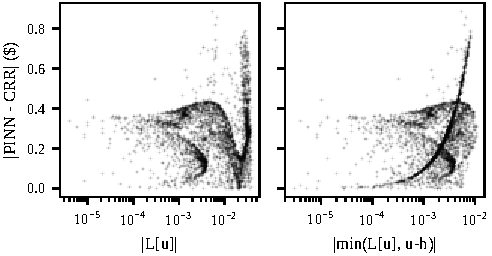
\includegraphics[width=\columnwidth]{figures/fig_p2_residual_vs_error.pdf}
\caption{N2, seed 0, 4000 pool points. Absolute price error against the raw residual $|L[u]|$ (left) and the LCP residual (right). The raw residual stays in a narrow band for any error; the LCP residual rises with the error.}
\label{fig:resid}
\end{figure}

\begin{table}[t]
\caption{Conformal bands, $n_{\mathrm{cal}}=800$, $n_{\mathrm{test}}=2000$, mean over 10 seeds $\times$ 20 splits. Width in \usd. Seed-to-seed std of coverage is at most \maxcovstd{}.}
\label{tab:conf}
\centering\footnotesize\setlength{\tabcolsep}{2.6pt}
\begin{tabular}{llrrrrrr}
\toprule
 & & \multicolumn{3}{c}{$\alpha=0.10$} & \multicolumn{3}{c}{$\alpha=0.05$}\\
Model & Score & Cov. & Width & Worst & Cov. & Width & Worst\\
\midrule
\tabinput{tables/table3_conformal.tex}
\bottomrule
\end{tabular}
\end{table}

\subsection{Conformal bands on PINN pricers}
Table~\ref{tab:conf} gives the main result. Marginal coverage is at its nominal level for every model and score, within 0.005. This holds for N2 too, despite its bias. The finite-sample guarantee does its job; the bias shows up as width. The PDE term shrinks the split band from \usd 19.43 (N0) to \usd 0.94 (N1) at $\alpha=0.10$, about 20 times. The choice of difficulty score matters. Normalising by $|L[u]|$ widens the N1 band (\usd 1.18 against \usd 0.94) and the N2 band (\usd 11.89 against \usd 10.05). It helps only N0, whose residual is large where it fails. For N2, the LCP residual gives \usd 9.01 against \usd 10.05 at the same coverage, but its worst bucket (0.71) is no better than split. Mondrian gives the narrowest bands and the best worst-bucket coverage (0.86 against 0.71 for split on N2). Fig.~\ref{fig:bucket} shows that split over-covers short tenors and under-covers deep in-the-money long tenors (0.71), while Mondrian keeps each bucket between 0.902 and 0.910 on average. Fig.~\ref{fig:slice} shows the bands on one slice: they contain the reference, but they are wide because the PINN sits above it.

\begin{figure}[t]
\centering
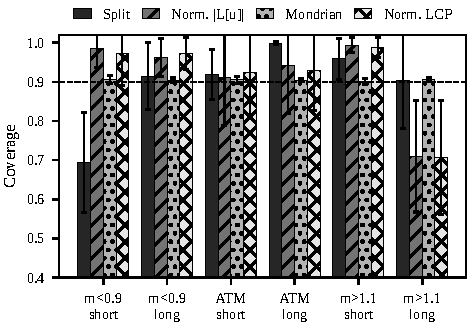
\includegraphics[width=\columnwidth]{figures/fig_p2_bucket_coverage_a10.pdf}
\caption{N2, $\alpha=0.10$, $n_{\mathrm{cal}}=800$: coverage per moneyness and tenor bucket (short: $\tau<0.4$), mean and std over 10 seeds. Dashed line: target 0.90. Only Mondrian is close to target in every bucket.}
\label{fig:bucket}
\end{figure}

\begin{figure}[t]
\centering
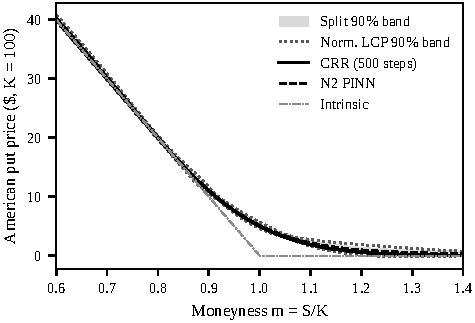
\includegraphics[width=\columnwidth]{figures/fig_p2_interval_slice_tau050.pdf}
\caption{American put at $\tau=0.5$, seed 0, $\alpha=0.10$. The split band (grey) and the LCP-normalised band (dotted) both contain the binomial price; the PINN lies above it, so the bands are wide and the lower edges fall below zero out of the money.}
\label{fig:slice}
\end{figure}

\subsection{Synthetic heteroscedastic check}
To isolate the score, we reuse a synthetic set with a known mean, noise standard deviation $0.01+0.12|m-1|$, difficulty $|m-1|$, $n_{\mathrm{cal}}=800$, $n_{\mathrm{test}}=2500$ and 50 seeds (Table~\ref{tab:p3}). Normalisation narrows the band (0.127 against 0.145 at $\alpha=0.10$) and raises coverage far from the money from 0.813 to 0.854. The fitted $\kappa$ is \kappafit{}, while the true ratio of slope to intercept is 12, so the adaptation is only partial. With homoscedastic noise, split coverage is 0.903 ($\alpha=0.10$) and 0.953 ($\alpha=0.05$).

\begin{table}[t]
\caption{Synthetic heteroscedastic data, 50 seeds. Width in $u$ units. Near: $|m-1|\le0.25$; far: $|m-1|>0.25$.}
\label{tab:p3}
\centering\footnotesize\setlength{\tabcolsep}{3.5pt}
\begin{tabular}{llrrrr}
\toprule
$\alpha$ & Score & Cov. & Width & Near & Far\\
\midrule
\tabinput{tables/table4_p3.tex}
\bottomrule
\end{tabular}
\end{table}

\subsection{Static arbitrage of prices and band edges}
We run the project's arbitrage checker on a put chain with $S=100$, strikes 60 to 140 in steps of 2.5 and ten expiries from 0.1 to 1 year, with tolerance $10^{-6}$ (Table~\ref{tab:p4}). Bands come from split 0, $n_{\mathrm{cal}}=800$, $\alpha=0.10$. The PINN prices break strike convexity in 12\% (N1) and 26\% (N2) of checkable triples. A constant split band keeps the convexity and calendar rates of the point price, since it only adds a term linear in $K$, but its lower edge raises monotonicity violations from 0.010 to 0.059. Bands of varying width add violations. About a third of lower edges are negative. The calendar check is not a valid condition for European puts: the exact Black-Scholes chain fails it in 27\% of cases. We apply no repair.

\begin{table}[t]
\caption{Static-arbitrage violation rates on a synthetic put chain (mean of 10 seeds). Put-call parity is not applicable to a put-only chain.}
\label{tab:p4}
\centering\footnotesize\setlength{\tabcolsep}{3pt}
\begin{tabular}{lrrrr}
\toprule
Series & Monot. & Convex & Calendar & Price${<}0$\\
\midrule
\tabinput{tables/table5_p4.tex}
\bottomrule
\end{tabular}
\end{table}

\section{Discussion}
\emph{Why keep the PINN if it loses on MAE?} It needs no labels, and it degrades gently outside any labelled region, where kernel and polynomial ridge fail (Table~\ref{tab:base}). It also exposes a residual for free. With a conformal layer, even a biased PINN gives bands with valid marginal coverage. The cost of the bias is width, so a better PINN gives narrower bands at once, as N1 against N0 shows.

\emph{Which residual?} The residual should measure distance from the conditions that define the solution. For a European option that is $L[u]=0$. For an American option it is the LCP (\ref{eq:lcp}), and $|L[u]|$ is not zero at the true solution in the exercise region. The LCP residual fixes this and is a much better error proxy. Still, Mondrian buckets beat it on conditional coverage here, so the two ideas can be combined in future work.

\emph{The N2 bias.} N2 is above the reference almost everywhere, also deep out of the money where early exercise hardly matters. We did not tune N2 after seeing these numbers. Candidate causes are the fixed loss weights and the boundary at $m=0$, where our code imposes the European value $e^{-r\tau}$ rather than the American value 1. We have not tested these causes.

\emph{What the data cannot show.} The project holds one Yahoo Finance snapshot of 4054 quotes from 13 Aug 2026 for SPX, NDX, NVDA and AAPL. One snapshot cannot support a time-ordered calibration and test split, so we report no market coverage. Real quotes also carry bid-ask noise and are not exchangeable across dates.

\section{Conclusion}
We placed split, normalised and Mondrian conformal bands on European and American PINN pricers. Marginal coverage held for every model, including a biased American PINN. The PDE loss shrank the European band about 20 times. Labelled regressors remain more accurate in-sample.

The difficulty score must match the problem. The raw PDE residual is a poor score for the American put, and the complementarity residual is a good one. Future work will fix the N2 bias, build a dated market panel for real coverage tests, project band edges onto arbitrage-free prices, and put a band on the exercise boundary $S^*(\tau)$.

\section*{Acknowledgment}
\DIFdelbegin \DIFdel{The authors thank }\DIFdelend Dr. Manish Kumar Tiwari \DIFdelbegin \DIFdel{for guidance. AI-use disclosure: }\DIFdelend \DIFaddbegin \DIFadd{supervised this project, and we thank him for his guidance. Use of AI: Grok Bot, }\DIFaddend an AI assistant\DIFdelbegin \DIFdel{(Grok Bot) wrote }\DIFdelend \DIFaddbegin \DIFadd{, produced }\DIFaddend the experiment scripts, \DIFdelbegin \DIFdel{drew }\DIFdelend the figures and \DIFdelbegin \DIFdel{drafted the text of all sections; the authors reviewed, revised }\DIFdelend \DIFaddbegin \DIFadd{first drafts of every section. We checked, edited }\DIFaddend and verified all \DIFdelbegin \DIFdel{content and take responsibility for it}\DIFdelend \DIFaddbegin \DIFadd{of it, and we are responsible for the content}\DIFaddend .

\bibliographystyle{IEEEtran}
\DIFdelbegin %DIFDELCMD < \bibliography{references}
%DIFDELCMD < %%%
\DIFdelend \DIFaddbegin \bibliography{references_ieeeabbrv}
\DIFaddend 

\end{document}
